\section{Examples of process-tensor workflows}
\label{sec:pt-workflows}

With the theory and programming interface of the previous sections in place, we now turn to physical examples. 
We demonstrate how the reduced system evolves, what the probability of a multi-round experimental record is, how operators at different times are correlated, and what changes when the intervention itself carries a persistent quantum memory. 
The following examples reproduce or adapt established open-system and quantum-information protocols; each is obtained by changing only the instruments contracted with a common \texttt{ProcessTensor}. 
We give a brief physical motivation and the core code that produces the figures; complete walkthroughs are in the \href{https://gauthameshwar.github.io/ProcessTensors.jl/stable/}{package documentation}.

%%%%%%%%%%%%%%%%%%%%%%%%%%%%%%%%%%%%%%%%%%%%%%%%%%%%%%%%%%%%
\subsection{Reduced dynamics of a central spin}
\label{subsec:workflow-central-spin}

A first use of a process tensor is the familiar "recover the reduced dynamics of a system after its environment has been eliminated".  
We borrow, for this purpose, the fully polarised central-spin benchmark used by Cygorek \emph{et al.} to demonstrate ACE for a non-Gaussian spin environment~\cite{Cygorek2022}.  
A central spin-$1/2$, $\mathbf S$, interacts isotropically with $N$ noninteracting bath spins $\mathbf s_k$,
%
\begin{equation}
    H_S=H_E=0,
    \qquad
    H_{SE}
    =
    \sum_{k=1}^{N}
    \frac{J_k}{\hbar^2}\,
    \mathbf S\!\cdot\!\mathbf s_k,
    \qquad
    J_k=\frac{J}{N}.
    \label{eq:central-spin-hamiltonian}
\end{equation}
%
\begin{figure}[H]
    \centering
    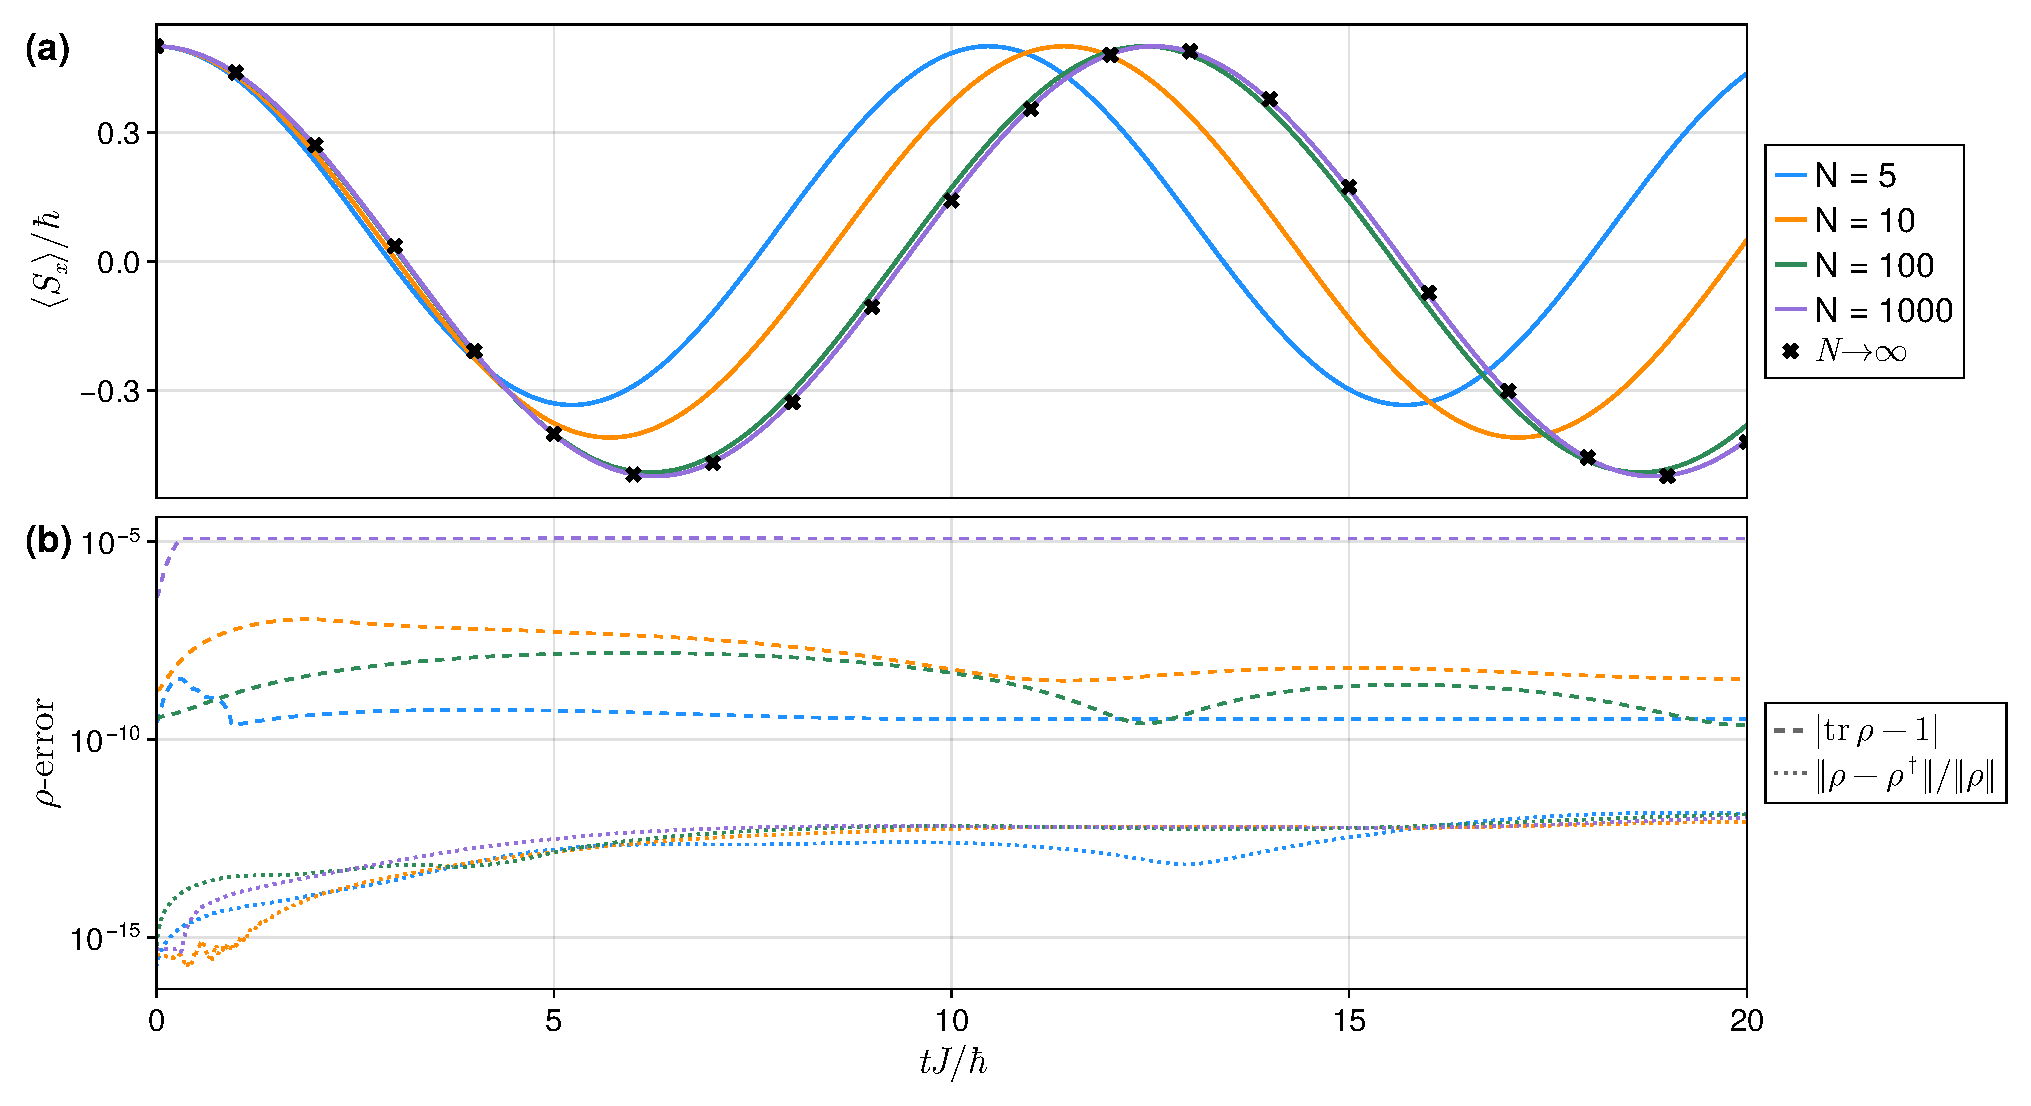
\includegraphics[width=\linewidth]{figures/central_spin.pdf}
    \caption{%
        \textbf{(a)~Fully polarised central-spin dynamics.}
        Reduced dynamics of the system spin coupled to a finite number of bath spins.
        Finite baths of the model in Eq.~\eqref{eq:central-spin-hamiltonian} approach the analytical $N\rightarrow\infty$ precession in Eq.~\eqref{eq:central-spin-limit} as $N$ increases.
        \textbf{(b)~Trace and hermiticity errors of $\rho$.}
        The lower panel records $\lvert\operatorname{Tr}\rho-1\rvert$ and $\lVert\rho-\rho^\dagger\rVert/\lVert\rho\rVert$.
    }
    \label{fig:workflow-central-spin}
\end{figure}
%
The system is initially polarised along $+x$, while every bath spin begins along $+z$. 
Keeping $\sum_kJ_k=J$ fixed prevents the interaction energy scale from growing with the number of modes. 
The system and bath spins have no free Hamiltonian that leads to a unitary evolution in their own subspace. 
Since neither subsystem has a free Hamiltonian, all non-trivial dynamics are generated by the system–bath interaction and depend on the initially polarised bath state. 
% When we have just a few bath spins, we might observe non-trivial dynamics where a spin mode in the bath can couple with the central spin and produce non-trivial coupling with another spin mode in the same bath, despite no real coupling existing between the two bath spins. 
For finite \(N\), back-action from the central spin generates correlations among bath spins even though they do not interact directly. 
These mediated correlations produce finite-size deviations from the collective precession. 
However, in the limit $N\rightarrow\infty$, the bath experiences vanishing back-action and produces a static effective magnetic field, giving
%
\begin{equation}
    \frac{\langle S_x(t)\rangle}{\hbar}
    \longrightarrow
    \frac{1}{2}\cos\!\left(\frac{Jt}{2\hbar}\right).
    \label{eq:central-spin-limit}
\end{equation}
%
Each bath spin is supplied to \texttt{ACE()} as an independent \texttt{SpinMode}.
Once their joint influence has been compressed into a PT-MPO, the microscopic bath is no longer needed for the reduced calculation. 
%
\begin{juliacode}[
    caption={Independent bath spins assembled into an ACE process tensor.},
    label={lst:workflow-central-spin},
]
bath_sites = siteinds("S=1/2", N)
bath_sites_L = liouv_sites(bath_sites)

modes = SpinMode[]
for k in 1:N
    rho_k = to_dm(MPS([bath_sites[k]], ["Up"]))
    coupling = OpSum()
    coupling += J / N, "Sx", 1, "Sx", 2
    coupling += J / N, "Sy", 1, "Sy", 2
    coupling += J / N, "Sz", 1, "Sz", 2
    push!(
        modes,
        spin_mode([bath_sites_L[k]], OpSum(), rho_k; coupling=coupling),
    )
end
bath = spin_bath(modes)

process_tensor = build_process_tensor(
    system; method=ACE(cutoff=1e-10),
    environment=bath, dt=0.01, nsteps=nsteps,
)

trajectory = evolve(process_tensor, rho_S0)
Sx_t = [real(tr(Sx * density_matrix(rho)))
        for rho in trajectory.states_hilbert]
\end{juliacode}
%

%%%%%%%%%%%%%%%%%%%%%%%%%%%%%%%%%%%%%%%%%%%%%%%%%%%%%%%%%%%%
\subsection{Repeated Ramsey measurements with active reset}
\label{subsec:workflow-ramsey}

Reduced dynamics observes the system without intervening. 
A process tensor also predicts the joint statistics of an experiment in which measurements and controls are applied repeatedly. 
We illustrate this using Ramsey interferometry, introduced originally as a separated-oscillatory-field spectroscopy protocol~\cite{Ramsey1950}, and now ubiquitous in qubit characterisation. 
This choice is also motivated by recent studies of temporally correlated circuit noise generated by multimode spin--boson environments~\cite{FigueroaRomero2021RB,Gandhari2026RBSpinBoson}. 
The qubit is coupled through $Z$ to a thermal bosonic environment described by the pure-dephasing spin--boson model,
%
\begin{equation}
    H_E=\sum_k\omega_k b_k^\dagger b_k,
    \qquad
    H_{SE}=Z\sum_k \sqrt{J(\omega_k)}(b_k+b_k^\dagger),
    \qquad
    J(\omega_k)=2\alpha\omega_k e^{-\omega_k/\omega_c},
    \label{eq:ramsey-spin-boson}
\end{equation}
%
which is a standard model of structured dephasing noise~\cite{Leggett1987SpinBoson}. 
The continuum is discretised into thermal oscillator modes and compressed once with \texttt{ACE()}. 

The experimental protocol performed on the qubit is as follows: the qubit is initially prepared in $\rho_{\mathrm r}=|+\rangle_x\langle+|$, evolves for a fixed Ramsey time, and is read out with the POVM
%
\begin{equation}
    E_x^{(\eta)}
    =\frac{1}{2}\bigl(\mathbb I+x\eta\sigma_x\bigr),
    \qquad
    x\in\{-1,+1\},
    \qquad
    0\leq\eta\leq1.
    \label{eq:ramsey-povm}
\end{equation}
%
Here, \(\eta\) is the effective measurement visibility (sharpness), quantifying how reliably the Ramsey readout distinguishes the two \(X\)-basis outcomes. 
A POVM element fixes the outcome probability but not the state supplied to the following round.  
We therefore combine the readout with an outcome-independent active reset and use the causal-break operation
%
\begin{equation}
    \mathcal A_x^{\mathrm{MR}}(\rho)
    =\operatorname{Tr}\!\left[E_x^{(\eta)}\rho\right]\rho_{\mathrm r},
    \qquad
    =|\rho_{\mathrm r}\rangle\!\rangle
    [\mathcal A_x^{\mathrm{MR}}]
      \langle\!\langle E_x^{(\eta)}|.
    \label{eq:ramsey-measure-reset}
\end{equation}
%
Each outcome map is CP and trace-non-increasing, while their sum is the CPTP replacement channel
%
\begin{equation}
    \sum_x\mathcal A_x^{\mathrm{MR}}(\rho)
    =\operatorname{Tr}(\rho)\rho_{\mathrm r}.
    \label{eq:ramsey-complete-instrument}
\end{equation}
%
Measure-and-reprepare causal breaks are central to the operational definition and experimental reconstruction of non-Markovian processes ~\cite{Pollock2018Framework,White2020,White2022ProcessTomography}. 
A causal break introduced in the system will ensure no information of the qubit's previous states before this break affects its future dynamics through the qubit itself. 
If any correlation is observed in the following dynamics, it should come from the process tensor of the environment. 

\texttt{ProcessTensors.jl} does not yet provide a dedicated POVM container in v0.3.0. 
Each outcome map in Eq.~\eqref{eq:ramsey-measure-reset} is instead assembled from two single-leg instruments: an output-leg \texttt{observable\_measurement} of \(E_x^{(\eta)}\) and an input-leg \texttt{state\_preparation} of \(\rho_{\mathrm r}\). 
The package overloads \texttt{*} for this purpose. 
Provided the two instruments have opposite prime levels---one with \(\operatorname{plev}=0\) and one with \(\operatorname{plev}=1\)---their product is a \texttt{ProductInstrument}, a two-leg object inserted at a single evolve slot of an \texttt{InstrumentSeq}. 
If we perform this POVM measurement and reset three times, we obtain the joint probability \(p(x_1,x_2,x_3)\) of the record \(\lvert x_1\rangle_x\), \(\lvert x_2\rangle_x\), \(\lvert x_3\rangle_x\).
%
\begin{juliacode}[
    caption={POVM-and-reset \texttt{ProductInstrument}s for three Ramsey readouts.},
    label={lst:workflow-ramsey},
]
eta = 0.90
rho_r = to_dm(MPS(system_sites, ["+"]))

effects = Dict(x => (OpSum() + (0.5, "Id", 1) + (0.5 * x * eta, "X", 1)) for x in (-1, 1))
instruments = Dict(
    x => observable_measurement(effects[x]) * state_preparation(rho_r)
    for x in (-1, 1)
)

for record in Iterators.product((-1, 1), (-1, 1), (-1, 1))
    seq = default_schedule(process_tensor)
    seq += state_preparation(rho_r), 0
    for (k, x) in zip(readout_steps, record)
        seq += instruments[x], k
    end
    seq += trace_out(), process_tensor.nsteps
    probabilities[record] = real(evaluate_process(process_tensor, seq))
end
\end{juliacode}
%

Evaluating the process tensor for each of the above records, the returned scalar is the joint probability 
%
\begin{equation}
    p(x_1, x_2, x_3)
    =
    \operatorname{Tr}\!\left[
        \mathcal T
        \bigl[
        \mathcal A_{x_3}^{\mathrm{MR}},
        \mathcal A_{x_2}^{\mathrm{MR}},
        \mathcal A_{x_1}^{\mathrm{MR}},
        \mathcal P_{\rho_{\mathrm r}}
        \bigr]
    \right].
    \label{eq:ramsey-record-probability}
\end{equation}
%
\begin{figure}[H]
    \centering
    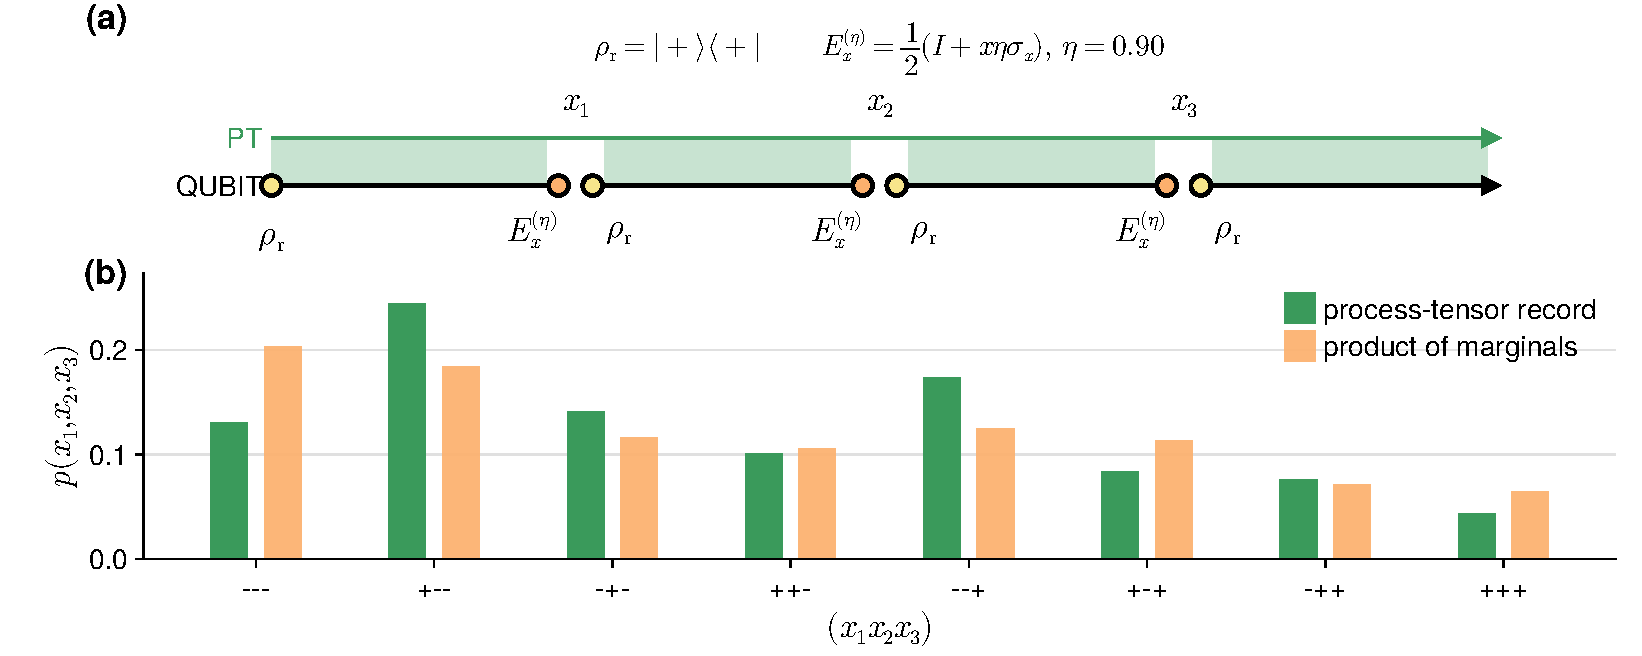
\includegraphics[width=\linewidth]{figures/ramsey_readouts.pdf}
    \caption{%
        \textbf{(a)~Timeline of the Ramsey readout protocol.}
        Three repeated readouts of the thermally dephasing qubit in Eq.~\eqref{eq:ramsey-spin-boson}, each followed by the same active reset, Eq.~\eqref{eq:ramsey-measure-reset}.
        The time exposed to the environment between each prepare and measure is the same for all three readouts.
        The green fill between the PT and QUBIT line depicts constant interaction between them.
        \textbf{(b)~Outcome-record probabilities $p(x_1,x_2,x_3)$.}
        For some three-shot records the process-tensor probabilities do not coincide with the products of the single-round marginals, indicating correlations between successive readouts.
    }
    \label{fig:workflow-ramsey}
\end{figure}
%
The eight probabilities in Fig.~\ref{fig:workflow-ramsey} are non-negative and sum to unity, as required by Eq.~\eqref{eq:ramsey-complete-instrument}.
% Since the time for which the qubit is exposed to the noisy environment between each prepare and measure is the same for all three readouts, we would expect the joint probability \(p(x_1,x_2,x_3)\) to be the product of the single-round probabilities \(p(x_1)p(x_2)p(x_3)\). 
For a memoryless process, the active reset makes the three identically timed rounds independent, so that the joint distribution factorises as \(p(x_1,x_2,x_3)=\prod_jp(x_j)\).
Deviations from the product of the measured single-round marginals therefore reveal information retained by the environment across causal breaks.
Thus, this is an operational signature of non-Markovianity. 

%%%%%%%%%%%%%%%%%%%%%%%%%%%%%%%%%%%%%%%%%%%%%%%%%%%%%%%%%%%%
\subsection{Multi-time correlations in a spin environment}
\label{subsec:workflow-correlations}

Correlation functions at multiple times govern response theory, noise spectroscopy, and multidimensional spectroscopy. 
In a non-Markovian problem they cannot, in general, be reconstructed from the reduced trajectory alone because the first operator insertion changes the subsequent joint system--environment evolution. 
PT-MPO calculations of such correlations have been developed for strongly coupled spin chains and structured baths~\cite{Fux2023TensorNetworkChains}, and have since been used in process-tensor approaches to nonlinear spectroscopy ~\cite{deWit2025Spectroscopy}. 
We take a minimal two-spin analogue so that every result can also easily be checked against direct joint evolution,
%
\begin{equation}
    H_S=S_x,
    \qquad
    H_E=S_x,
    \qquad
    H_{SE}=S_z\otimes S_z,
    \label{eq:correlation-spin-model}
\end{equation}
%
with the system initially in $|\!\downarrow\rangle$ and the environment in $|\!\uparrow\rangle$.

For $t_2\geq t_1$, the ordered correlation is
%
\begin{equation}
    C_{AB}(t_2,t_1)
    =
    \operatorname{Tr}_{SE}\!\left[
        (A\otimes\mathbb I_E)U_{2:1}(B\otimes\mathbb I_E)
        U_{1:0}\rho_{SE}(0)U_{1:0}^{\dagger}U_{2:1}^{\dagger}
    \right].
    \label{eq:exact-two-time-correlation}
\end{equation}
%
Thus $B$ is inserted from the left at $t_1$, the resulting operator is propagated to $t_2$, and $A$ closes the final leg. 
The order is reversed when $t_1>t_2$, while coincident insertions are combined on the same temporal leg. 
These cases are encoded by \texttt{two\_time\_correlation\_seq}, so a complete grid reuses one process tensor:
%
\begin{juliacode}[
    caption={Two-time correlation grid from one stored process tensor.},
    label={lst:workflow-correlations-grid},
]
Czz = [
    evaluate_process(
        process_tensor,
        two_time_correlation_seq(
            process_tensor, (sigma_z, n2), (sigma_z, n1);
            rho0=rho_S0,
        ),
    )
    for n1 in time_indices, n2 in time_indices
]
\end{juliacode}
%

For \(t_2>t_1\), the helper translates Eq.~\eqref{eq:exact-two-time-correlation} into instruments: \(\rho_S(0)\) is prepared at the first input, \(B\) is inserted as a left action at \(t_1\), \(A\) is inserted as a left action at \(t_2\), and a terminal \texttt{trace\_out} realises the partial trace. 
On a five-step process with \((n_2,n_1)=(3,1)\), the resulting schedule is
%
\begin{julialistingpair}[
    caption={Instrument sequence for \(C_{zz}(t_3,t_1)\) on a five-step process.},
    label={lst:workflow-correlations-seq},
]
    \begin{juliacode}[paired]
seq = two_time_correlation_seq(
    process_tensor, (sigma_z, 3), (sigma_z, 1);
    rho0=rho_S0,
)
println(seq)
    \end{juliacode}
    \begin{juliaoutput}[paired]
InstrumentSeq(default=IdentityOperation, nsteps=5, 4 explicit entries)
  tstep=0 => StatePreparation{MPO{Hilbert, Nothing}}
  tstep=2 => LeftRightOperator{MPO{Hilbert, Nothing}, MPO{Hilbert, Nothing}}
  tstep=4 => LeftRightOperator{MPO{Hilbert, Nothing}, MPO{Hilbert, Nothing}}
  tstep=5 => TraceOut
    \end{juliaoutput}
\end{julialistingpair}
%
The default identity fills the idle slots \(1\) and \(3\).  
The left-action at \texttt{tstep=2} is \(B=\sigma_z\) at \(t_1\), and that at \texttt{tstep=4} is \(A=\sigma_z\) at \(t_2\).
If \(t_1>t_2\), the early insertion becomes a right action; if \(t_1=t_2\), the two operators are multiplied on the same temporal leg.

Several expectations follow without solving the dynamics.  
Hermiticity and $\sigma_z^2=\mathbb I$ give
%
\begin{equation}
    C_{zz}(t,t)=1,
    \qquad
    C_{zz}(t_2,t_1)^*=C_{zz}(t_1,t_2),
    \label{eq:czz-structure}
\end{equation}
%
so the real and imaginary parts are respectively symmetric and antisymmetric under $t_1\leftrightarrow t_2$.  
The equal-time cross-correlations instead follow from
%
\begin{equation}
    \sigma_z\sigma_x=i\sigma_y,
    \qquad
    \sigma_x\sigma_y=i\sigma_z.
    \label{eq:cross-correlation-diagonal}
\end{equation}
%
Consequently, the real parts of the corresponding equal-time correlations vanish. 
The numerical grids in Fig.~\ref{fig:workflow-correlations} reproduce these correlation properties faithfully.
%
\begin{figure}[H]
    \centering
    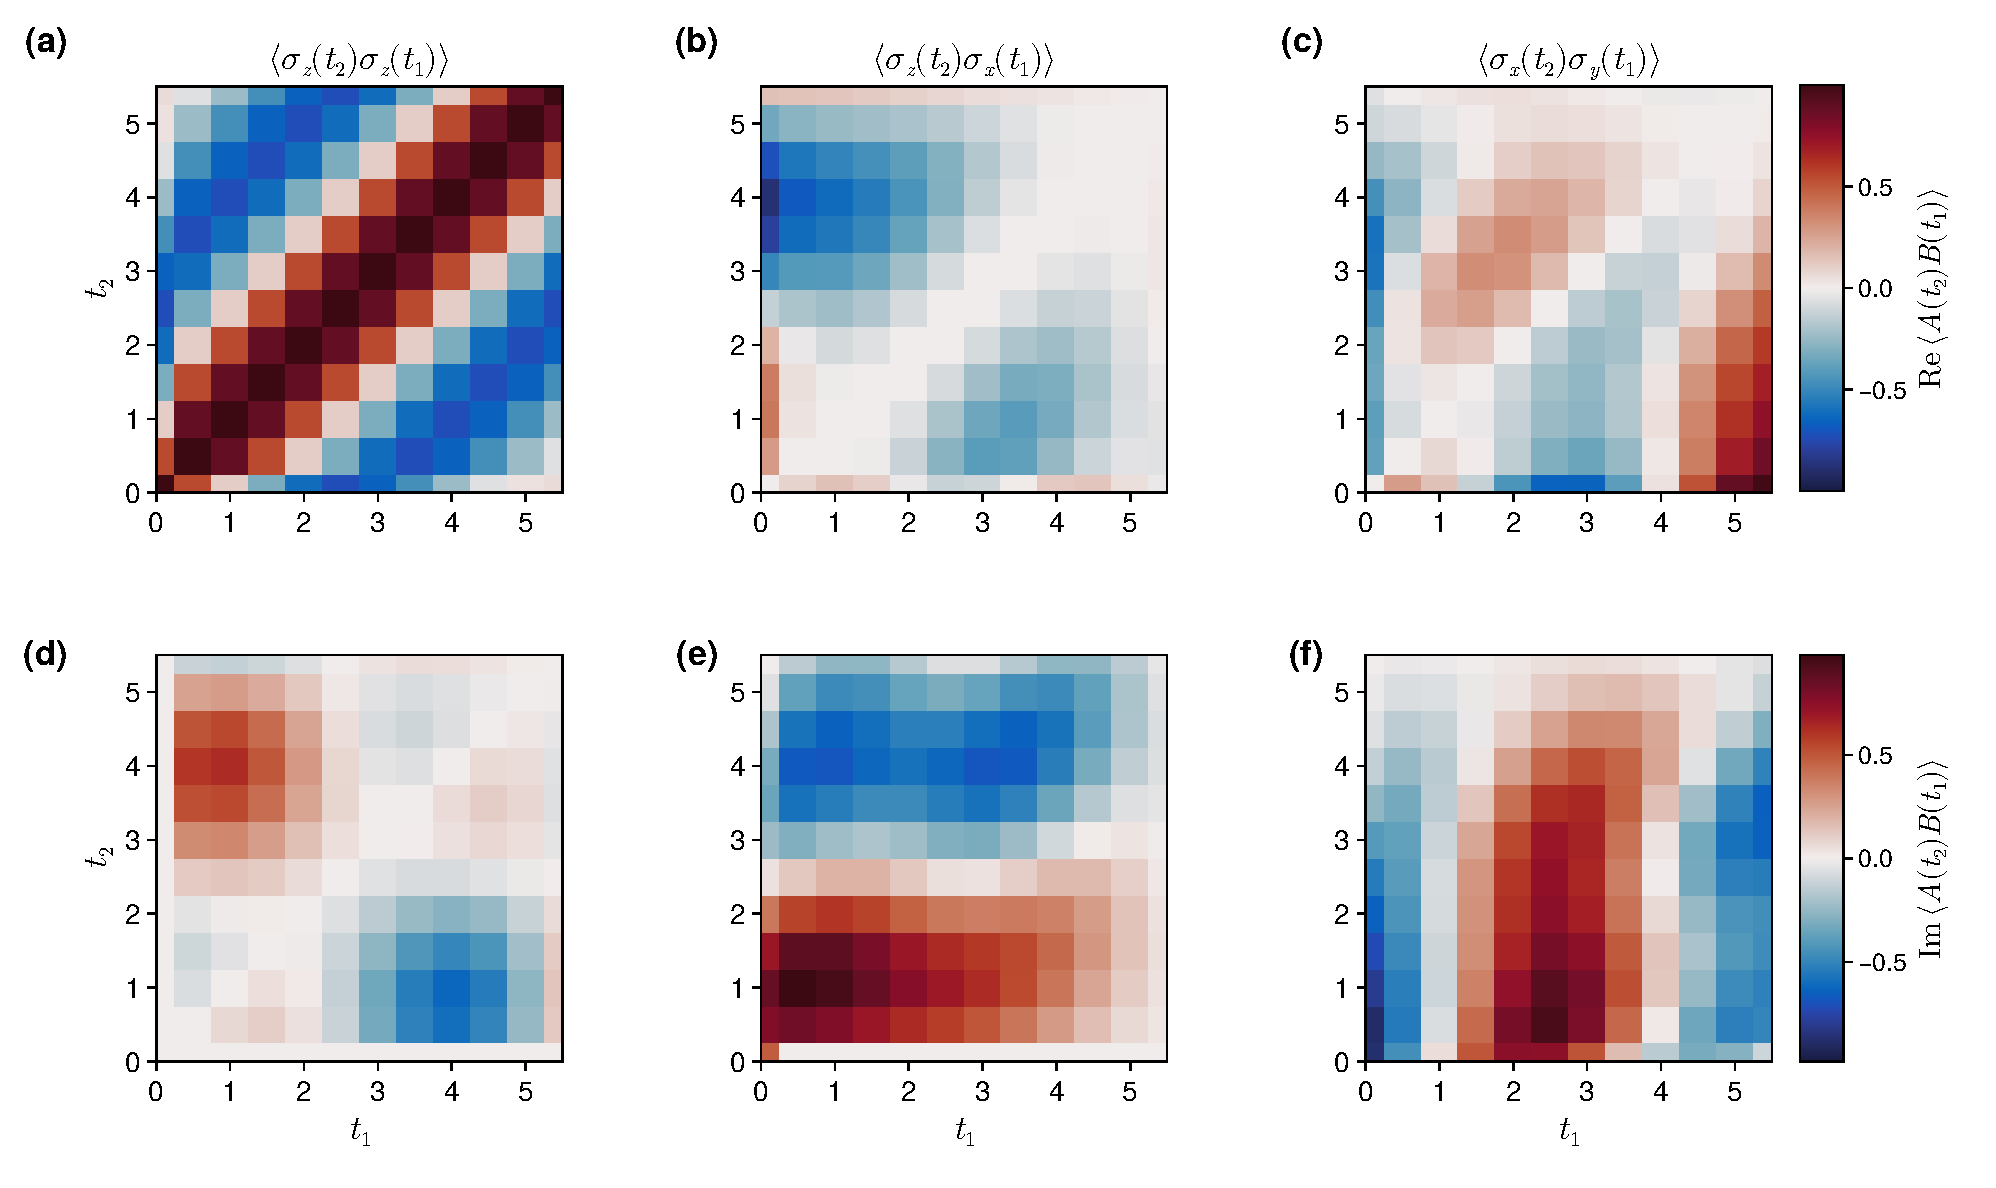
\includegraphics[width=\linewidth]{figures/multitime_correlations.pdf}
    \caption{%
        \textbf{Two-time spin correlations from a reused process tensor.}
        Panels (a)--(c) show the real parts of $C_{zz}$, $C_{zx}$, and $C_{xy}$ for the two-spin model in Eq.~\eqref{eq:correlation-spin-model}; (d)--(f) show the corresponding imaginary parts.
        The autocorrelation (a) has a unit real diagonal and the conjugate symmetry of Eq.~\eqref{eq:czz-structure} in (d); the cross-correlation diagonals follow Eq.~\eqref{eq:cross-correlation-diagonal}.
        Every pixel is obtained by changing only the two operator-insertion times of the same stored process tensor.
    }
    \label{fig:workflow-correlations}
\end{figure}
%

%%%%%%%%%%%%%%%%%%%%%%%%%%%%%%%%%%%%%%%%%%%%%%%%%%%%%%%%%%%%
\subsection{Memory-assisted control with a quantum tester}
\label{subsec:workflow-tester}

The previous experiments repeatedly removed the system's local memory. 
We finally consider the opposite setting, in which the intervention deliberately retains a quantum memory. 
Quantum testers and combs were introduced to describe the most general probing strategies for channels used over several times, including protocols in which an ancilla persists between uses~\cite{Chiribella2008MemoryDiscrimination, Chiribella2009}. 
Such memory-assisted strategies are particularly natural for correlated circuit noise, whose implications for randomized benchmarking have been analysed in Refs.~\cite{FigueroaRomero2021RB,Gandhari2026RBSpinBoson}.

We return to the thermal spin--boson process of Eq.~\eqref{eq:ramsey-spin-boson}, but attach an isolated ancillary qubit $A$ to the noisy processor qubit $S$.  
The protocol is as follows: first SWAP the system and ancilla to store the logical state in $A$, then apply a $Z_A$ gate only on the ancilla while it is parked away from the bath, and then do the second SWAP to retrieve it. 
The persistent ancillary wire turns this sequence into a temporally correlated tester. 
%
\begin{juliacode}[
    caption={SWAP--phase--SWAP tester sequence for memory-assisted control.},
    label={lst:workflow-tester},
]
memory = tester(ancilla_sites, rho_A0)

U_SA = op("SWAP", only(system_sites), only(ancilla_sites))
U_A = op("Z", only(ancilla_sites))
joint_U_SA = joint_unitary(U_SA, system_sites, ancilla_sites)
local_U_A = tester_unitary(U_A, ancilla_sites)

controls = TesterSeq(nsteps=process_tensor.nsteps)
controls += joint_U_SA, store_step
controls += local_U_A, phase_step
controls += joint_U_SA, retrieve_step

trajectory = evolve(
    process_tensor, rho_S0;
    tester=memory, tester_seq=controls, return_joint=true,
)
\end{juliacode}
%
\begin{figure}[H]
    \centering
    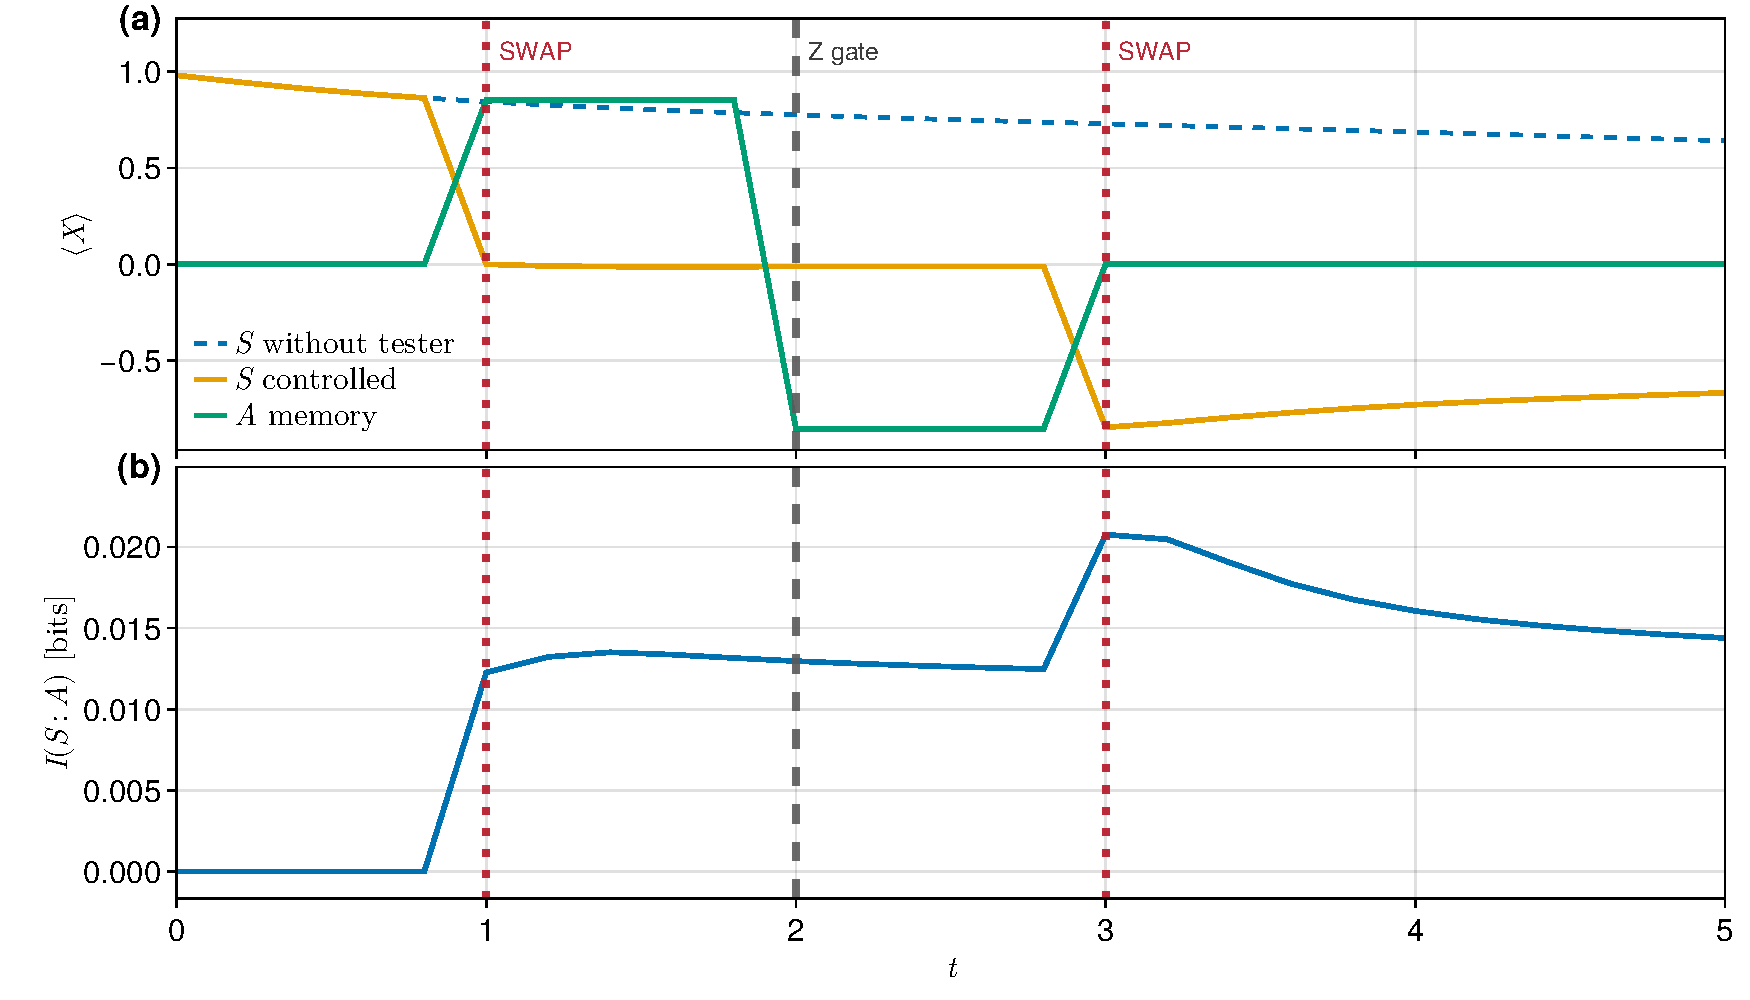
\includegraphics[width=\linewidth]{figures/tester_instrument.pdf}
    \caption{%
        \textbf{(a)~Transverse magnetisation of the SWAP--phase--SWAP protocol.}
        The first SWAP transfers $\langle X\rangle$ from the noisy processor $S$ to the isolated ancilla $A$, the $Z_A$ gate reverses its sign, and the second SWAP returns it; the uncontrolled system continues to dephase on the processor.
        \textbf{(b)~System--ancilla correlation.}
        The first SWAP parks the logical state in $A$ while the environment retains the processor history; later evolution and the retrieval SWAP convert part of that history into $I(S{:}A)\approx 0.02$ bits.
        The small magnitude reflects the weak-coupling parameters used here.
    }
    \label{fig:workflow-tester}
\end{figure}
%

The output of evolving a PT-MPO with a tester contains the reduced states $\rho_S(t)$ and $\rho_A(t)$ by default. 
The joint trajectory $\rho_{SA}(t)$ is obtained by setting \texttt{return\_joint=true}. 
We quantify the total correlations of that joint state by the quantum mutual information
%
\begin{equation}
    I(S{:}A)
    =S(\rho_S)+S(\rho_A)-S(\rho_{SA}),
    \qquad
    S(\rho)=-\operatorname{Tr}\!\left(\rho\log_2\rho\right).
    \label{eq:tester-mutual-information}
\end{equation}
%
The panels of Fig.~\ref{fig:workflow-tester} follow this protocol. 
With no tester, the processor dephases under the thermal bath. 
The first SWAP parks the logical state in the isolated ancilla, while the environment retains correlations with the history of the processor. 
Subsequent evolution and the final SWAP convert part of that environmental history into system--ancilla correlations, so the observed $I(S{:}A)$ is a signature of the process tensor rather than of the joint gates alone. 
Its peak value of about $0.02$ bits is small because the spin--boson coupling used here is weak. 
The two memories remain distinct: environmental memory is compressed into the PT-MPO, whereas the experimenter's controllable memory is carried by the tester ancilla.

Taken together, these workflows move from an unobserved reduced trajectory to outcome-resolved causal breaks, operator insertions at two times, and finally a coherent intervention with its own memory.  
Their common implementation is the central design choice of \texttt{ProcessTensors.jl}: the expensive environment is encoded once, while the experiment is changed by replacing the instruments attached to its temporal legs.
